\documentclass{ucl_thesis}

%twoside for double page printing
\usepackage{graphics}
\usepackage{graphicx}
\usepackage{color}
\usepackage{verbatim}
\usepackage{algorithm}
\usepackage{algorithmic}
\newcommand{\theHalgorithm}{\arabic{algorithm}}
\usepackage[square]{natbib}

\usepackage[font=footnotesize,labelfont=bf,singlelinecheck=on]{caption}

\usepackage{amsmath}
% Uncomment this to activate the TikZ library, which is useful for fancy block-diagrams.
%    \usepackage{tikz}
%    \usetikzlibrary{positioning,arrows,shapes.misc}
\usepackage{multirow}

%\numberwithin{algorithm}{chapter}
%\usepackage{epsf}
\usepackage{fancyvrb}

%\documentclass[12pt,a4paper]{article}
%\usepackage[utf8]{inputenc}
\usepackage[english]{babel}
%\usepackage{amsmath}
%\usepackage{amsfonts}
%\usepackage{amssymb}
%\usepackage{graphicx}
%usepackage[left=2cm,right=2cm,top=2cm,bottom=2cm]{geometry}
%
%\usepackage[]{natbib}

%% LISTINGS
\usepackage{color}
\usepackage{listings}
\definecolor{mygreen}{rgb}{0,0.6,0}
\definecolor{mygray}{rgb}{0.5,0.5,0.5}
\definecolor{mymauve}{rgb}{0.58,0,0.82}
\definecolor{purple}{rgb}{0.28,0.23,0.5}
\lstdefinestyle{customcpp}{
  belowcaptionskip=1\baselineskip,
  breaklines=true,
  frame=L,
  xleftmargin=\parindent,
  language=C++,
  showstringspaces=false,
  basicstyle=\footnotesize\ttfamily,
  keywordstyle=\bfseries\color{green},
  commentstyle=\itshape\color{purple},
  identifierstyle=\color{blue},
  stringstyle=\color{orange},
  numbers        = left,
  stepnumber     = 5,
}
%%

%% figure template
\newcommand{\myfig}[6]{%
\begin{figure}[h!]\centering%
	\begin{minipage}[b]{0.49\linewidth}\centering%
		\includegraphics[width=\textwidth]{#2}%
		\caption{#3}%
		\label{fig:#1}%
	\end{minipage}%
	\begin{minipage}[b]{0.49\linewidth}\centering%
		\includegraphics[width=\textwidth]{#5}%
		\caption{#6}%
		\label{fig:#4}%
	\end{minipage}%
\end{figure}%
}
%%

%% shortcuts
%Malcolm added some custom commands here - you can make your own!
\newcommand{\vect}[1]{\boldsymbol{#1}}
\newcommand{\figref}[1]{(Fig. \ref{#1})}
\def\etal{{et~al.}}
\def\ie{{\it i.e.,\ }}
\def\etc{{\it etc.,\ }}
\def\eg{{\it e.g.,\ }}
\def\vs{{\it vs.\ }}
%%

\author{Aron Monszpart}
\title{Super-resolution hand-held scanning}
\def \supervisor {Dr. Gabriel Brostow}
\date{September 2013}

\begin{document}

\bibliographystyle{plainnat}
\maketitle
\numberwithin{algorithm}{chapter}
\setcounter{page}{1}
\pagenumbering{roman}
\pagestyle{plain}

% Notice how the star "*" is used throughout LaTex to modify the normal behavior. For example, \section* instead of \section 
% tells LaTex NOT to number this section.


\newpage
\section*{Abstract}
I've done some stuff
%\input{abstract.tex}


\newpage
\section*{Acknowledgements}
Dr. Gabriel Brostow, Dr Neill Campbell, Dr. Oisin Mac Aodha, Fabrizio Pece, Malcolm Reynolds, Clement Godard, Peter Rennert and the UCL PRISM group

%\setcounter{tocdepth}{2}
\tableofcontents
\listoffigures
%\listoftables
%\listofalgorithms
\newpage

\setcounter{page}{1}
\pagenumbering{arabic}
\pagestyle{plain}

\chapter{Introduction and Background} 
\label{chp:background}
	\begin{itemize}	
		\item Motivation
		\item Overview of approach
		\begin{itemize}
			\item Calibration
			\item Low resolution 3D reconstruction
			\item Pose estimation of new input
			\item Mesh subdivision and 2D projection
			\item Depth upsampling
			\item Mesh enhancement by backprojection
		\end{itemize}
	\end{itemize}

\chapter{Related work} 
\label{chp:related_work}

\section{Calibration}
\label{sec:lit_calib}

One of the initial steps of the setup of every multi-camera system has to be calibration. The expression calibration can be interpreted with several meanings. In this document we refer to calibration as the preprocessing step that captures the characteristics of the physical recording system accounting for, amongst others, inaccuracies in the physical manufacturing processes of the cameras. A successful calibration enables a correspondence to be calculated between data captured at the same time with the different cameras. This correspondence is data dependent in the case of depth cameras, and thus calculated every frame.\\
A wider interpretation of calibration includes the calculation of a nearly global position of the recording system. It usually is incorporated by the relative position estimation between the observed scene and the recording system, which can be viewed as global in case the global position of the observed scene is known. \\

Most previous works targeting to develop a highly accurate calibration system use the pinhole-camera model. 
\citep{Zhang00}

$\left(\begin{array}{ccc}
		f_x & \gamma & c_x \\
		b & f_y & c_y \\
 		0 & 0 & 1 \\
	    \end{array} \right)$

http://burrus.name/index.php/Research/KinectCalibration


\section{Depth upsampling}
\citep{MatsuoFI13} \\

In \citep{Silberman:ECCV12} ... they give a very good kinect dataset for segmentation, use RANSAC and implement cross bilateral filtering

\section{Kinect fusion papers}
\citep{Chen:2013:Scalable_volumetric}
\section{planned}

	\begin{enumerate}
		\item 3D reconstruction using Multi-view stereo
		\begin{itemize}
			\item Curless and Levoy
			\item Rusinkiewicz
			\item Szeliski
			\item Agarwal
			\item Snavely
			\item Seitz
			\item Furukawa and Ponce
			\item Strecha
			\item etc. from literature review (got good marks for it)
			\item Kim et al: Scene reconstruction from High Spatio-Angular Resolution Light Fields (Siggraph '13)
		\end{itemize}

		\item 3D reconstruction using RGB-D
		\begin{itemize}
			\item Voxelgrid based
			\begin{itemize}
				\item Newcombe: Kinect fusion
				\item Whelan: Kintinuous and other loop closure papers
				\item Vladlen: Dense scene reconstruction with points of interest
				\item etc.
			\end{itemize}

			\item Height-field based, layered
			\begin{itemize}
				\item Adaptive voxelgrid based, scene scale aware (Freiburg)
				\item etc.
			\end{itemize}

			\item Point based
			\begin{itemize}
				\item Damien Lefloch
				\item etc.
			\end{itemize}

			
		\end{itemize}
			
 		\item Pose estimation
		\begin{itemize}
			\item some ICP references
			\item Gyro papers
			\item MVS already earlier
		\end{itemize}
		
		\item Upsampling
		\begin{itemize}
			\item RGB superresolution
			\item Depth superresolution
			\begin{itemize}
				\item Non-guided
				\begin{itemize}
					\item Learning based
						\begin{itemize}
							\item Mac Aodha et al. '12
							\item etc.
						\end{itemize}
					\item Other
					\begin{itemize}
						\item Hornacek et al.: Depth Super Resolution by Rigid Body Self-Similarity in 3D, CVPR '13
						\item etc.
					\end{itemize}
				\end{itemize}
				
				\item Guided
				\begin{itemize}
					\item Joint Bilateral
					\begin{itemize}
						\item Yang '07
						\item etc.
					\end{itemize}
					\item MRF based
					\begin{itemize}
						\item Diebel and Thrun
						\item Schuon et al.
						\item Park et al. '11
						\item Choi et al. '12
						\item Shen and Cheung CVPR '13 (Layer Depth Denoising and Completion for Structured-Light RGB-D Cameras)
						\item etc.
					\end{itemize}
					
					\item Spatio-temporal filtering
					
				\end{itemize}
			\end{itemize}
		\end{itemize}
		
		\item Commercial 3D scanners
		\begin{itemize}
			\item MVS based: Photosynth, Adobe, etc.
			\item Laser scanner systems (industrial)
			\item Kinect based: Scanec, Reva, ReconstructMe, ...
		\end{itemize}
		
		\item Seen/used calibration references
		\item Subdivision references
		\item Efficient raycasting references
		\item (+ Categorize all the ref e-mails from Gabriel, Oisin, Reading groups, etc.)
	
	\end{enumerate}

\chapter{MySystem} 
\label{chp:my_system}

\section{Calibration}
\label{sec:calibration}

What is calibration, pinhole camera model, different notations (oulu, \citep{Zhang00}, etc.), 
with IR, without IR
USB bus problems, overlayed image

% Input rgb and depth
\begin{figure}[h!]\centering
    \begin{minipage}[b]{0.49\linewidth}
        \includegraphics[width=\textwidth]{/home/bontius/workspace/cpp_projects/KinfuSuperRes/SuperRes-NI-1-5/build/out/imgs_20130725_1809/img8_00000001.png}
        \caption{Input RGB}
    \end{minipage}
    \begin{minipage}[b]{0.49\linewidth}
        \includegraphics[width=\textwidth]{/media/Storage/Dropbox/UCL/project/results/presentation_300713/dep8_00000001.png}
		\caption{Input depth}
    \end{minipage}
\end{figure}

% Simple alignment
\begin{figure}[h!]\centering
	\begin{minipage}[b]{0.49\linewidth}
		\includegraphics[width=\textwidth]{/media/Storage/Dropbox/UCL/project/results/presentation_300713/dep16AndRgb_00000001.png}
		\caption{No alignment}
	\end{minipage}
	\begin{minipage}[b]{0.49\linewidth}
		\includegraphics[width=\textwidth]{/media/Storage/Dropbox/UCL/project/results/presentation_300713/dep16AndRgb_00000000.png}
		\caption{"Built-in alignment"}
	\end{minipage}
\end{figure}


\begin{figure}[h!]\centering
    \begin{minipage}[b]{0.49\linewidth} \label{fig:ir}
        \includegraphics[width=\textwidth]{/media/Storage/Dropbox/UCL/project/results/presentation_300713/irAndDep8_00000001.png}
        \caption{Default IR and depth overlay}
    \end{minipage}
    \begin{minipage}[b]{0.49\linewidth}
        \includegraphics[width=\textwidth]{/media/Storage/Dropbox/UCL/project/results/presentation_300713/offsIrAndDep8_00000001.png}
        \caption{IR offset by radius of convolution kernel}
    \end{minipage}
\end{figure}

\begin{figure}[h!]\centering
        \includegraphics[width=\linewidth]{/home/bontius/workspace/cpp_projects/KinfuSuperRes/SuperRes-NI-1-5/build/out/imgs_20130725_1809/img8_00000001_mapped.png}
        \caption{Mapping from 640x480 depth to 1280x1024 RGB after calibration}
\end{figure}


default image, built in alignment image, good image\\
calibration papers, and their comparison of optimisation techniques\\
calibration with different sources (depth and acryl, ir, ellipses)\\
cuda mapping\\


\subsection{takeaway}
Ir image with and without projector\\
large checkerboard vs. small checkerboard\\
all positions (mosaic image?)\\

\section{Yang}

%\lstset{frame=single,language=C++,tabsize=1,basicstyle=\ttfamily\small,}
\lstset{style=customcpp}
\begin{lstlisting}
__device__ float yangRangeDist( float4 a, float4 b, float sigma )
{
    float mod = ( fabs(b.x - a.x) +
                  fabs(b.y - a.y) +
                  fabs(b.z - a.z)  ) / 3.f;
    return __expf(-mod / sigma);
}
template <typename T>
__global__ void
d_cross_bilateral_filterF( T *dOut, int w, int h, size_t outPitch,
                           float range_sigma, int r, bool onlyZeros = false )
{
    int x = blockIdx.x*blockDim.x + threadIdx.x;
    int y = blockIdx.y*blockDim.y + threadIdx.y;

    if (x >= w || y >= h) return;

    float sum = 0.f, factor = 0.f, t = 0.f;
    float4 guideCenter = tex2D( guideTex, x, y );
    T      centerPix   = fetchTexture<T>( x, y );

    // check for early exit
    if ( onlyZeros && (centerPix != 0.f) )
    {
        dOut[y * outPitch + x] = centerPix;
        return;
    }

    // estimate cost volume
    for ( int i = -r; i <= r; ++i )
    {
        for ( int j = -r; j <= r; ++j )
        {
            // read depth
            T curPix = fetchTexture<T>( x+j, y+i );
            // skip, if no data
            if ( onlyZeros && curPix == 0.f )
                continue;
            // read rgb
            float4 guidePix = tex2D( guideTex, x + j, y + i );
            // estimate weights
            factor = cGaussian[i + r] * cGaussian[j + r] *
                     yangRangeDist( guidePix, guideCenter, range_sigma );
            // accumulate
            t   += factor * curPix;
            sum += factor;
        }
    }
    if ( sum > 0.f )
        dOut[y * outPitch + x] = t / sum;
    else
        dOut[y * outPitch + x] = centerPix;
}

\end{lstlisting}

\section{Kinect Fusion}

\section{Combined pipeline}
My combined pipleine ( this is what I did, to get the data fro mhere to there. Draw attention to GPU implementations (get credit for it) )

%%% CHAPTER 5 %%%
\chapter{Validation / experiments}
\label{chp:validation}

%%% SECTION %%%
\section{Structure from motion} 
\label{sec:sfm}

% acerlit image
\myfig
{acerlit_1}
{/home/bontius/workspace/cpp_projects/KinfuSuperRes/thesis/img/acer_lit00706.jpg}
{A frame of video of backside of a monitor}
{acerlit_mesh}
{/home/bontius/workspace/cpp_projects/KinfuSuperRes/thesis/img/acer_lit01.png}
{Visual SFM 3D reconstruction of monitor} 

% oil bottle image
\begin{figure}[h!]\centering
	\begin{minipage}[b]{0.49\linewidth}\centering
		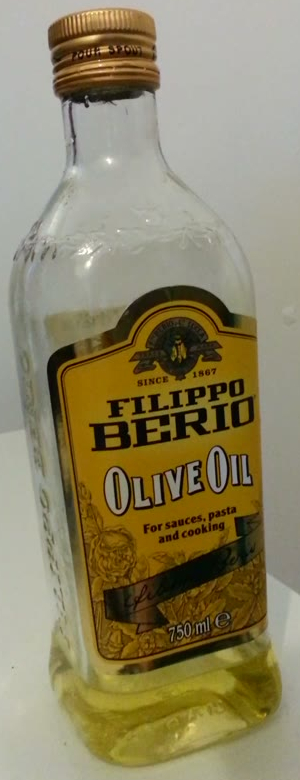
\includegraphics[height=5cm]{/home/bontius/workspace/cpp_projects/KinfuSuperRes/thesis/img/ob00003r2.jpg}
		\caption{A frame of video of oil bottle}
		\label{fig:ob_1}
	\end{minipage}
	\begin{minipage}[b]{0.49\linewidth}\centering
		
\includegraphics[height=5cm]{/home/bontius/workspace/cpp_projects/KinfuSuperRes/thesis/img/ob_mesh00.png}
		\caption{Visual SFM 3D reconstruction of oil bottle}
		\label{fig:ob_mesh}
	\end{minipage}
\end{figure}

%%% SECTION %%%
\section{Iterative joint bilateral upsampling with subpixel accurracy}
\label{sec:yang}

\begin{figure}[h!]\centering 
        \includegraphics[width=\linewidth]{/media/Storage/Dropbox/UCL/project/results/final/yang_checkerboard/yanged_nonflat.png}        
        \caption{Example run of implementation on checkerboard scene, results without and with texture after 50 iterations.}
        \label{fig:yang_checkerboard}
\end{figure}

In \figref{fig:yang_checkerboard} 



\chapter{Discussion} \label{chp:discussion}
    - come back to 3's experiments\\
    - interpret experiments\\
    - did you notice, that 2 were good, and 3rd was abd, remember what I sadi in 3.2, that kinfu does it's calibration...well ,that's crap here (threshold), it happend to be good for 2 sequences, but not their thirds \\
-     Pros, cons \\
- PFM format \\

\section{Limitations} \label{sec:limitations}
	- so if Kinfu is not reliable, say it! so if it does not work (pose) than \\
	- misalignment, few frames later, it's great \\
	- calibration \\
    - obvious (Yang on chessboard, it still does) \\
    - summarizing what I discovered \\
    
\section{Future work}
- Using segmentation \citep{Silberman:ECCV12} \\
- Occlusion \citep{Hoiem:2011} \\
- Learning based alignment and depth \citep{Herrera:LearnedJointMRF} \\

future work: I advocate Yang for the following reasons, or I discourage, since...or in some situations this, than that \\
Kinect \\
Yang \\
Grid recordings of monitor\\


%\section{System plan}
%	\begin{itemize}
%		\item Calibration
%			\begin{itemize}
%				\item Depth image based
%				\item IR image based
%				\item Undistort
%			\end{itemize}
%		\item Low resolution 3D reconstruction
%			\begin{itemize}
%				\item Multi View Stereo (VSFM, Bundler, Photosynth, etc.)
%				\item Kinect Fusion, PCL::Kinfu
%			\end{itemize}
%		\item Pose estimation of new input
%			\begin{itemize}
%				\item VSFM ( for RGB input )
%				\item ICP ( for RGB-D input )
%				\item Gyro+IMU (a noisy graph of acquired data)
%			\end{itemize}
%		\item Mesh subdivision (Linear, Butterfly, Catmull-Clark)
%		\item 2D projection
%			\begin{itemize}
% 				\item Raycasting using Octree
%				\item GLSL projection
%			\end{itemize}
%		\item Yang filtering
%			\begin{itemize}
%				\item Iterative Cross Bilateral filtering
%				\item Subpixel accurracy
%			\end{itemize}
%		\item Mesh enhancement by backprojection
%	\end{itemize}
%	
%\section{System design}
%	\begin{itemize}
%		\item Implementation details and takeaway experience of "System plan" elements
%		\item Merge into previous?
%	\end{itemize}
%	
%\section{Evaluation}
%	\begin{itemize}
% 	\item Experiments
%		\begin{itemize}
%			\item Calibration
%				\begin{itemize}
%					\item Kinect built in calibration
%					\item Bogouet calibration with and without lens distortion (PARAMETERS explained)
%					\item Undistort effectivity (project undistorted depth map to 3D)
%				\end{itemize}
%				
%			\item Filtering
%				\begin{itemize}
%					\item CrossBilateral filter vs. Bilateral
%					\item Yang vs. CrossBilateral (PARAMETERS explained)
%					\item Trilateral, Guided, Pixel Weighted Average Strategy (Garcia et al,ImProc, 2010) - {\bf IF there's time}
%				\end{itemize}
%			\item Kinect fusion related
%			\begin{itemize}
%				\item Kinfu vs. Kinfu w/ filtering turned OFF
%				\item Kinfu voxel grid resolution ($386^3$,$512^3$,$640^3$)
%				\item Kinfu + Yang( original kinect depth frames )
%				\item Kinfu + Yang( "arbitrary pose" )
%			\end{itemize}
%		\end{itemize}
%	\item Existing libraries used
%	\item Data capturing details
%	\item No existing datasets compared (no time)
%
%	\end{itemize}
%
%\section{Results}
%\begin{itemize}
%	\item Upsampling with original depth frames
%	\item Upsampling with simulated "arbitrary pose"
%
%	\item original yang images
%	\item subpixel refinement
%	
%	\item So, Yang is is not suitable for this resolution, it only could improve, when the input was much noisier
%	\item Different approaches can be plugged in to this framework to enhance depth
%\end{itemize}
%\section{Conclusions, Future work}
%	\begin{itemize}
%		\item 3D reconstruction improvements
%			\begin{itemize}
%				\item Improve on smoothing effect of voxel grid weights
%				\item Pose estimation improvements
%			\end{itemize}
%		\item RGB high-resolution capture, vsfm pose estimation 
%		\item Enhancement by best pose selection from input image collection for given pixel/region
%	\end{itemize}

\section{Used libraries}
NVIDIA bilateralfiltering sample
PCL
 pcl bilateral upsampling
 \citep{DCBGridStereo}
 

\section{References}
	...
	
\citep{Lowe04}

%\bibliographystyle{plainnat}
\bibliography{litrev}
	
\end{document}


